% Main paper: manuscript H1-H3 in simulation + causal real-data replay.
% Every number comes from \input{numbers} (research/figures/paper_main.py,
% generated from research/results/ only); every figure from figures/ (same script).
% Build: bash research/papers/main/build.sh
\documentclass[10pt,twocolumn]{article}
\usepackage[margin=0.75in]{geometry}
\usepackage{amsmath,amssymb}
\usepackage{graphicx}
\usepackage{booktabs}
\usepackage{xcolor}
\usepackage[hidelinks]{hyperref}
\usepackage{natbib}
\setcitestyle{authoryear,round}

\input{numbers}

\title{Keeping ``None of the Above'' in the Loop: Open-World, Causal Follow-Up Planning for Fading Transients, in Simulation and on Real ZTF Events}
\author{Joyce Malik\\ \small [Department], [Institution], India \quad \texttt{[email]}}
% TODO before submission: affiliation, email, co-authors.
\date{}

\begin{document}
\maketitle

\begin{abstract}
Information-driven follow-up planners for astronomical transients assume that the event belongs to a modeled class and that measurements can be taken whenever they are most informative. We test a planner that drops both assumptions. It keeps an explicit unmodeled hypothesis $h_0$, represented by a Gaussian process, in its posterior, and adds an opportunity-decay term to its utility. Three preregistered hypotheses were tested in a simulated constellation of eight Starlink satellites with real orbital visibility, with measurements strictly forward in time (\SimNEvents\ events per scenario). At a 5\% false-alarm rate, the planner's $P(h_0)$ detected \SimTprP\ of events from withheld classes, against \SimTprBthree\ for a classifier-entropy threshold, while closed-world information gain was confidently wrong on \SimCwWhBthreeAll\ of them. Removing the decay term reduced recovered amplitude information more for fast classes than for slow ones, although the effect was carried by kilonovae, reversed for flares and reversed under model error. The planner was not the fastest to identify modeled events: classifier-entropy sampling was. An adequacy term in the utility contributed nothing measurable. On \RealNEvents\ real ZTF transients replayed against the same fleet, a preregistered causal test confirmed four of five hypotheses: the planner was confidently wrong on \RealCCwWhP\ of real tidal disruption events, superluminous and SN~Ibn supernovae, against \RealCCwWhBthree\ for closed-world information gain, with an AUROC of \RealCAuc\ and supernova accuracy equal to the closed-world planner's; it could not be shown non-inferior in accuracy within 5 points. We also report a time-ordering error that affected our earlier results, and how correcting it changed them.
\end{abstract}


\section{Introduction}
Wide-field surveys discover more transients than follow-up resources can observe \citep{Bellm2019,Ivezic2019}, so the choice of \emph{which measurement to take next} is a planning problem. Expected information gain (EIG) about the class label \citep{Lindley1956,Chaloner1995} is the natural objective for that choice, but it makes two assumptions that fail exactly where follow-up matters most. It assumes the event belongs to one of the modeled classes, which is false for rare and new phenomena. And it treats measurements as interchangeable in time, while the epochs that separate fast transients vanish within hours to days.

We study a planner that drops both assumptions. Its posterior carries an explicit unmodeled hypothesis $h_0$, represented by a Gaussian process (GP), and its utility adds, to the class EIG, an adequacy term (the information a measurement carries about whether $h_0$ is true) and an opportunity-decay term (what is lost by waiting). We test three of its claims in a simulated low-Earth-orbit constellation with real orbital visibility, and the open-world claim again on real Zwicky Transient Facility (ZTF) events with the measurements replayed counterfactually. All hypotheses, analyses and selection rules were fixed in preregistration files committed before the test data were run. We report the failures with the same prominence as the successes.

\paragraph{A correction that shaped this paper.} An earlier version of our pipeline did not enforce a time arrow: an adaptive planner could measure at day~0.01 after it had measured at day~0.96. In the earlier real-data test runs, \CausalBugPct\ of the adaptive planners' measurement sequences went backwards in time at least once. Results from that version, including an earlier research note, compare strategies fairly but describe \emph{retrospective epoch selection}, not follow-up. Every result in Sections~\ref{sec:sim}--\ref{sec:real} is \emph{causal}: each measurement is strictly later than the one before. We report the retrospective numbers only for comparison, labelled as such.

\section{Method}\label{sec:method}
\paragraph{Belief.} For $K$ modeled classes with forward models $f_k(t;\theta)$, the planner holds an exact grid posterior over $(k,\theta)$; here $\theta$ is the amplitude (and, on real data, a two-band template). Measurements are Gaussian, $y\sim\mathcal N(f_k(t;\theta),\sigma_i^2)$, with $\sigma_i$ set by the instrument's limiting magnitude. The open-world posterior adds $h_0$, scored by the marginal likelihood of a zero-mean GP with a squared-exponential kernel, with a uniform prior over $\{1,\dots,K,h_0\}$.

\paragraph{Utility.} A candidate action $a$ is an (epoch, spacecraft) pair that is visible and strictly later than the last measurement. The planner P maximizes
\begin{equation}
U(a) = I(H_{1:K};Y_a) + \beta\, I(Z;Y_a) + \gamma\, D(a),
\end{equation}
where $I(H_{1:K};Y_a)$ is the closed-world class EIG, $Z=\mathbb 1[h_0]$, and both mutual informations are computed by exact one-dimensional quadrature over the predictive mixture. $D(a)$ is the posterior-weighted loss in squared signal-to-noise between measuring now and at the same spacecraft's next opportunity, a Fisher-information proxy for the per-class information decay. When $P(h_0)>0.9$ for two consecutive steps, P switches from discrimination to preservation and takes the earliest remaining epochs.

\paragraph{Baselines and ablations.} B0 measures at a fixed cadence (earliest feasible epoch). B1 re-implements the constellation's original Contract-Net auction score (geometric margin and sensitivity, no belief). B2 picks where the modeled classes' point-estimate predictions disagree most (classifier-entropy sampling, no likelihood marginalization). B3 is closed-world EIG, the key comparison. Two ablations remove one term of P each: P$_{\gamma=0}$ (no decay) and P$_{\beta=0}$ (no adequacy term; $h_0$ stays in the belief). Every strategy receives identical events, orbits, instruments, noise draws and budgets for a given seed.

\section{Simulation study}\label{sec:sim}
\paragraph{Setup.} Four modeled classes (kilonova, shock-cooling, GRB afterglow, M-dwarf flare) and three withheld classes never shown to any planner (an AT2018cow-like fast blue optical transient, a tidal disruption event, and a physically implausible brightening oscillation) are drawn uniformly. Their light curves are analytic shapes chosen to match each class's qualitative timescales, \emph{not} published templates. Amplitudes are log-uniform on $[5,20]$ in units of the 20th-magnitude noise floor. Eight Starlink satellites, propagated with SGP4 from real element sets, carry instruments with limiting magnitudes 19, 20 or 21 assigned at random, and see a random sky position only when it is not occulted by the Earth. Each strategy gets five measurements over 16 log-spaced epochs from 0.01 to 20~days. Scenarios: Nominal; Crowding (half of all epoch--satellite cells unavailable); and Model error (each modeled class's timescale misspecified by 30\% in the belief, but not in the truth).

\paragraph{Hypotheses (preregistered).} H1: P reaches posterior $\geq 0.95$ on the true modeled class in less median time than every baseline, with the same measurement budget (one-sided paired Wilcoxon, Holm over four baselines). H2: removing the decay term reduces the information recovered about the true class's amplitude more for fast classes (kilonova, shock cooling, flare) than for the slow class (GRB afterglow) (stratified bootstrap). H3: at a 5\% false-alarm rate on modeled events, P's $P(h_0)$ detects more withheld events than a threshold on the closed-world posterior entropy of B3 (paired bootstrap). Only the Nominal scenario decides pass or fail; the others are reported. The decay weight $\gamma$ and the GP length scale were tuned on validation seeds only, by a rule fixed beforehand (maximum mean log score of P).

\paragraph{Results.} Validation selected $\gamma=\SimGamma$ (the largest value in the grid) and a GP length scale of \SimLengthscale\,d. On the \SimNEvents\ Nominal test events (\SimNModeled\ modeled, \SimNWithheld\ withheld), H1 \SimHOneVerdict, H2 and H3 \SimHTwoVerdict. Table~\ref{tab:sim} lists every strategy in every scenario.

\paragraph{H1, identification speed: refuted.} P reached posterior $\geq0.95$ on the true class after a median of \SimTtiP\ and did so for \SimIdP\ of modeled events (Fig.~\ref{fig:tti}). It was faster than fixed cadence (which identified only \SimIdBzero), the auction baseline (median \SimTtiBone) and closed-world EIG (\SimTtiBthree; Holm $p$ \SimHolmBthree\ for each). It was not faster than classifier-entropy sampling B2, whose median was \SimTtiBtwo. The paired test favours P over B2 (Holm $p=\SimHolmBtwo$) only because B2 identified just \SimIdBtwo\ of events and unidentified events rank last. Pair by pair, P was slower in \SimSlowerBtwo\ of pairs and faster in \SimFasterBtwo. The preregistered criterion requires a shorter median, so H1 fails. P beats closed-world EIG here for an unflattering reason: under causality B3 greedily jumps to late, high-contrast epochs and uses only \SimObsAllBthree\ of its 5 measurements, against \SimObsAllP\ for P.

\begin{figure}[t]
\centering
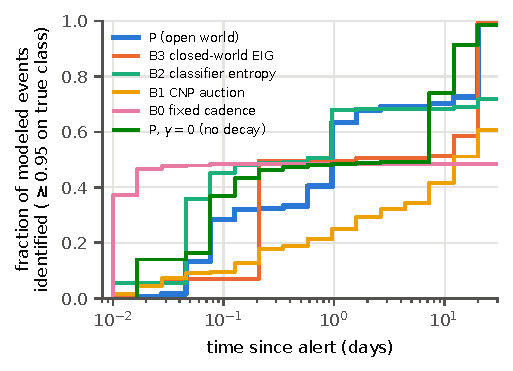
\includegraphics[width=\columnwidth]{generated/figures/fig1_tti.pdf}
\caption{H1. Cumulative fraction of modeled events whose posterior on the true class has reached 0.95, by time since alert (Nominal, test). B2 identifies the events it identifies earliest; P identifies almost all of them but later; closed-world EIG (B3) defers many identifications to the final epochs.}
\label{fig:tti}
\end{figure}

\paragraph{H2, irreversibility: supported, with caveats.} Removing the decay term reduced the information recovered about the true class's amplitude by \SimHtwoFast\ nats on fast classes and \SimHtwoSlow\ on the slow GRB afterglow, a difference of \SimHtwoEst\ \SimHtwoCI. The effect is carried by kilonovae (\SimDeltaKilonova) and, less, shock cooling (\SimDeltaShock); for the fastest class, the M-dwarf flare, the decay term \emph{lost} information (\SimDeltaFlare; Fig.~\ref{fig:decay}). It also reversed under model error, where the misspecified timescales mislead the urgency estimate (\SimHtwoModelErrorEst\ \SimHtwoModelErrorCI).

\begin{figure}[t]
\centering
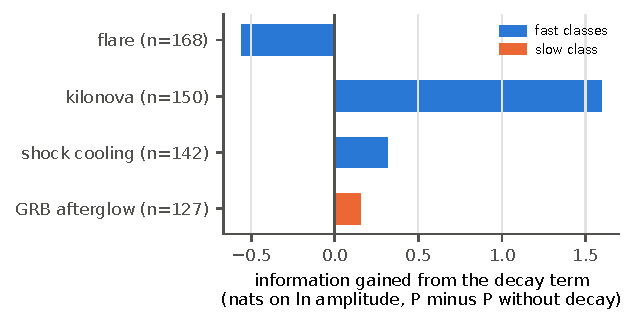
\includegraphics[width=\columnwidth]{generated/figures/fig2_decay.pdf}
\caption{H2. Per-class information about the true amplitude gained by the decay term (P minus P without it), Nominal test. Positive for kilonova and shock cooling, near zero for the slow class, negative for flares.}
\label{fig:decay}
\end{figure}

\paragraph{H3, open-world detection: supported.} At a 5\% false-alarm rate on modeled events, P's $P(h_0)$ detected \SimTprP\ of withheld events; thresholding the closed-world posterior entropy of B3 detected \SimTprBthree\ (difference \SimHthreeEst\ points, 95\% CI \SimHthreeCI; Fig.~\ref{fig:rocsim}). AUROCs were \SimAucP\ for $P(h_0)$ against \SimAucBthree\ (B3 entropy) and \SimAucBtwo\ (B2 entropy). Entropy computed on P's own measurements did no better (\SimAucPown), so the gain comes from the hypothesis, not from P's choice of measurements. Without $h_0$, closed-world EIG was confidently wrong on \SimCwWhBthreeAll\ of withheld events; P on \SimCwWhPAll, with no false ``unknown'' calls on modeled events (\SimFaP) and the same modeled accuracy as B3 (\SimAccModPAll). H3 held in all three scenarios, but model error is the predicted failure mode: P then called \SimFaPModelError\ of modeled events unknown and its modeled accuracy fell to \SimAccModPModelError\ (B3: \SimAccModBthreeModelError).

\begin{figure}[t]
\centering
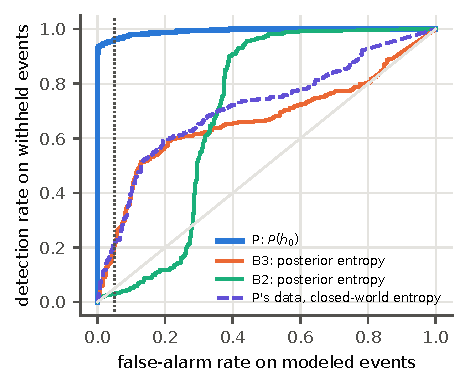
\includegraphics[width=\columnwidth]{generated/figures/fig3_roc_sim.pdf}
\caption{H3. ROC for separating withheld from modeled events (Nominal, test). Dotted line: the preregistered 5\% false-alarm operating point.}
\label{fig:rocsim}
\end{figure}

\paragraph{Ablations.} Removing the adequacy term changed nothing measurable: P$_{\beta=0}$ flagged \SimFlagNoAdeq\ of withheld events (P: \SimFlagP) with AUROC \SimAucAblNoAdeq\ (P: \SimAucAblP). Removing the decay term mattered: P$_{\gamma=0}$ took \SimObsAllNoDecay\ measurements instead of \SimObsAllP, flagged \SimFlagNoDecay, and was confidently wrong on \SimCwWhNoDecayAll\ of withheld events. In this setting the decay term's main effect on open-world detection is to stop the planner from spending its horizon too early, which gives $h_0$ enough data.

\begin{table*}[t]
\centering\scriptsize
\caption{Simulation test results (1000 events per scenario). Acc.\ mod.: accuracy on modeled events (\%); CW: confident-wrong rate (\%) on unmodeled (withheld) and modeled events; $\bar n_{\rm obs}$: measurements used of 5; log score: mean log probability of the true outcome (closed-world strategies cannot express ``withheld'' and are floored at $10^{-6}$).}
\label{tab:sim}
\begin{tabular}{llrrrrr}
\toprule
Scenario & Strategy & Acc.\ mod. & CW unmod. & CW mod. & $\bar n_{\rm obs}$ & log score \\
\midrule
Nominal & P (open world) & 100 & 6 & 0 & 4.2 & -0.19 \\
 & B3 closed-world EIG & 100 & 97 & 0 & 2.8 & -5.71 \\
 & B2 classifier entropy & 88 & 69 & 0 & 4.9 & -5.82 \\
 & B1 CNP auction & 80 & 75 & 0 & 3.2 & -5.92 \\
 & B0 fixed cadence & 79 & 1 & 0 & 5.0 & -5.92 \\
 & P, $\gamma=0$ (no decay) & 99 & 31 & 0 & 3.6 & -0.87 \\
 & P, $\beta=0$ (no adequacy) & 100 & 6 & 0 & 4.3 & -0.20 \\
\midrule
Crowding & P (open world) & 99 & 14 & 0 & 4.0 & -0.43 \\
 & B3 closed-world EIG & 100 & 94 & 0 & 3.0 & -5.82 \\
 & B2 classifier entropy & 94 & 80 & 0 & 4.8 & -5.88 \\
 & B1 CNP auction & 86 & 71 & 0 & 3.1 & -5.97 \\
 & B0 fixed cadence & 76 & 1 & 0 & 5.0 & -6.03 \\
 & P, $\gamma=0$ (no decay) & 100 & 31 & 0 & 3.4 & -0.96 \\
 & P, $\beta=0$ (no adequacy) & 99 & 14 & 0 & 4.1 & -0.43 \\
\midrule
Model error & P (open world) & 87 & 21 & 8 & 3.9 & -1.21 \\
 & B3 closed-world EIG & 99 & 96 & 1 & 2.9 & -6.11 \\
 & B2 classifier entropy & 81 & 29 & 4 & 5.0 & -6.32 \\
 & B1 CNP auction & 82 & 72 & 1 & 3.2 & -6.29 \\
 & B0 fixed cadence & 77 & 1 & 0 & 5.0 & -6.25 \\
 & P, $\gamma=0$ (no decay) & 93 & 26 & 6 & 3.4 & -1.32 \\
 & P, $\beta=0$ (no adequacy) & 86 & 21 & 8 & 3.9 & -1.21 \\
\bottomrule
\end{tabular}

\end{table*}


\section{Real-data replay}\label{sec:real}
\paragraph{Setup.} We replay spectroscopically classified ZTF Bright Transient Survey events \citep{Fremling2020,Perley2020} detected after the fleet existed, against the same Starlink satellites propagated from element sets archived at each event's date. Modeled classes are SN~Ia, SN~II and SN~Ibc, with empirical $g$- and $r$-band templates built only from events detected before 2020; tidal disruption events, superluminous supernovae and SN~Ibn are the real unmodeled population. Truth at any epoch is a GP interpolation of the real light curve; only the planner's measurements are simulated, and no epoch after the last real detection is offered. Each pointing returns simultaneous $g$ and $r$ fluxes, and each class likelihood includes its template population scatter (model discrepancy, $\kappa$ times the scatter). The events are split by date into validation (older half) and test (newer half).

\paragraph{Protocol.} The configuration (two bands, discrepancy $\kappa=0.5$, GP length scale 5\,d) was chosen on the validation split by a preregistered rule, and five hypotheses were fixed: P is less often confidently wrong than B3 on unmodeled events (H1); $P(h_0)$ ranks unmodeled above modeled events (H2, AUROC $>0.5$); P is not more than 5 points more often confidently wrong than B3 on supernovae (H3) and not more than 5 points less accurate (H5); and colour raises the AUROC over a single-band arm on the same events (H4). Each must pass on all three noise seeds (stratified paired bootstrap, $10^4$ resamples). The test events (\RealNEvents: \RealNModeled\ supernovae, \RealNWithheld\ unmodeled) had been used twice before, in the retrospective analyses; this causal run is a declared third look.

\paragraph{Results.} Table~\ref{tab:real} gives both versions side by side. With causal measurements, H1--H4 pass and H5 fails. Closed-world EIG was confidently wrong on \RealCCwWhBthree\ of real unmodeled transients (retrospectively \RealRCwWhBthree), the auction baseline B1 on \RealCCwWhBone, and P on \RealCCwWhP. P labelled \RealCFlagP\ of unmodeled events as unknown, and its AUROC was \RealCAuc\ (Fig.~\ref{fig:rocreal}).

\begin{table*}[t]
\centering\scriptsize
\caption{Real ZTF replay, preregistered test results per noise seed: estimate [95\% CI]; $^\times$ = criterion not met on that seed. CW: confident-wrong rate; $\Delta$ = P minus B3, or colour minus single-band arm for H4. Causal (v3) is this paper's result; retrospective (v2) let planners measure earlier epochs after later ones and is shown for comparison only.}
\label{tab:real}
\begin{tabular}{lll@{\hspace{4pt}}l}
\toprule
& Seed & Causal (v3) & Retrospective (v2) \\
\midrule
H1 $\Delta$CW unmod. & 1 & -0.49 [-0.60, -0.36] & -0.60 [-0.72, -0.49] \\
 & 2 & -0.42 [-0.55, -0.30] & -0.67 [-0.77, -0.56] \\
 & 3 & -0.36 [-0.48, -0.25] & -0.60 [-0.73, -0.48] \\
\addlinespace
H2 AUROC $P(h_0)$ & 1 & +0.81 [+0.76, +0.86] & +0.80 [+0.75, +0.85] \\
 & 2 & +0.81 [+0.76, +0.86] & +0.80 [+0.75, +0.85] \\
 & 3 & +0.79 [+0.73, +0.84] & +0.77 [+0.71, +0.82] \\
\addlinespace
H3 $\Delta$CW mod. & 1 & -0.05 [-0.09, -0.01] & +0.00 [-0.06, +0.07]$^\times$ \\
 & 2 & -0.04 [-0.08, +0.00] & +0.04 [-0.03, +0.10]$^\times$ \\
 & 3 & -0.03 [-0.07, +0.01] & +0.06 [-0.01, +0.12]$^\times$ \\
\addlinespace
H4 $\Delta$AUROC colour & 1 & +0.19 [+0.13, +0.24] & +0.19 [+0.14, +0.24] \\
 & 2 & +0.18 [+0.12, +0.23] & +0.21 [+0.16, +0.27] \\
 & 3 & +0.24 [+0.18, +0.30] & +0.15 [+0.10, +0.20] \\
\addlinespace
H5 $\Delta$acc.\ mod. & 1 & +0.01 [-0.05, +0.07]$^\times$ & -0.08 [-0.14, -0.02]$^\times$ \\
 & 2 & +0.03 [-0.04, +0.09] & -0.06 [-0.13, +0.00]$^\times$ \\
 & 3 & -0.01 [-0.08, +0.05]$^\times$ & -0.08 [-0.14, -0.01]$^\times$ \\
\addlinespace
\bottomrule
\end{tabular}

\end{table*}

\begin{figure}[t]
\centering
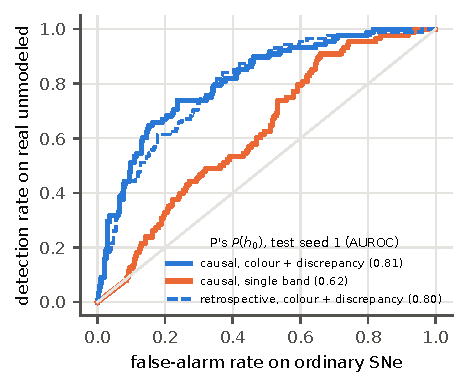
\includegraphics[width=\columnwidth]{generated/figures/fig4_roc_real.pdf}
\caption{Real data: ROC of the open-world planner's $P(h_0)$ separating real unmodeled transients (TDE, SLSN, SN~Ibn) from ordinary supernovae, test seed 1. Colour plus model discrepancy is what makes $h_0$ usable; enforcing causality leaves the curve almost unchanged.}
\label{fig:rocreal}
\end{figure}

\paragraph{What causality changed.} The retrospective runs failed H3 and H5: P paid for its safety on unknowns with more confident errors and lower accuracy on ordinary supernovae. Causally, H3 passes, the false-``unknown'' rate on supernovae falls from \RealRFaP\ to \RealCFaP, and P's supernova accuracy (\RealCAccModP) matches B3's (\RealCAccModBthree). H5 still fails, narrowly: on two seeds the lower confidence bound falls just below $-5$ points, so we cannot rule out a small loss. The cost moved to the unknowns: P flags \RealCFlagP\ of them, against \RealRFlagP\ retrospectively. The mechanism is the measurement budget. With a time arrow, one-step utilities jump to a late, informative epoch and forfeit the earlier ones: P used \RealCObsP\ of its 5 measurements on average (B3 \RealCObsBthree, the fixed-cadence B0 \RealCObsBzero), against \RealRObsP\ when it could go back in time. Fewer measurements make every posterior less confident, which removes confident errors on both populations, and with them some of P's detections.


\section{Discussion}\label{sec:disc}
\paragraph{What holds up.} Across all three studies, the robust result is the open-world \emph{posterior}. Keeping $h_0$ lets the planner say ``none of the above'', and it says so far more reliably than a threshold on closed-world uncertainty. In simulation this held in every scenario. On real data it held across three noise seeds and three looks at the test set, retrospective and causal. Closed-world planners are confidently wrong on most genuinely unmodeled transients; the open-world planner on a small fraction.

\paragraph{Two ways to say ``unknown''.} The Bayesian decision and the conformal one fail differently. The Bayesian $h_0$ made the fewest confident errors on real unknowns but has no false-alarm guarantee. The conformal threshold certified its false-alarm rate on fresh supernovae and, with lookahead, raised supernova accuracy above the closed-world planner's, at the price of more confident errors on unknowns. It also works on top of any planner, including a closed-world one. The choice between them is a choice of which error is costlier, and both beat closed-world planning on the unknowns.

\paragraph{What does not.} Two parts of the proposed utility did not earn their place. The adequacy term $\beta I(Z;Y_a)$, which targets measurements that test whether $h_0$ is true, made no measurable difference. An earlier toy study with retrospective sampling already suggested that planning with $h_0$ adds little beyond having it in the posterior. The decay term helped, but mainly by stopping greedy, myopic information gain from jumping to a late, high-contrast epoch and forfeiting the rest of its budget. Its benefit to fast classes was carried by kilonovae, reversed for flares (whose signal is gone before any epoch at which the proxy can act), and reversed when the forward models were wrong. And the planner was not the fastest identifier: a cheap disagreement heuristic identified the events it could identify sooner. A one-step utility has no notion of a horizon. The simple lookahead term of Section~\ref{sec:conf} used more of the budget and raised accuracy, but did not reliably improve the detection of unknowns; principled non-myopic planning remains open.

\paragraph{What the time-ordering error taught us.} Letting planners measure backwards in time did not bias the comparison between strategies, since every strategy had the same freedom, but it changed the conclusions. Retrospectively, all planners used their full budget; causally, adaptive planners used about half. With fewer measurements every posterior is less confident. That removed confident errors on both known and unknown events, turned the open-world planner's failed supernova-cost hypothesis (H3) into a pass, and cut the share of unknowns it flagged from \RealRFlagP\ to \RealCFlagP. A planner that can revisit the past cannot be evaluated as a follow-up planner. We recommend that benchmarks for sequential follow-up check the time order of every chosen sequence explicitly.

\paragraph{Limitations.} The simulated classes are analytic shapes chosen to match qualitative timescales, not published models, and amplitude is their only physical parameter, so H2 measures information about amplitude only. The decay term is a squared-signal-to-noise proxy, not the per-class information decay it stands for. There is no slew or exposure cost, a single band in simulation, geometric visibility only (no link budget), and a centralized planner, so the distributed-allocation hypothesis of the original proposal is untested. The decay weight was selected at the edge of its validation grid. On real data, measurements are resampled from interpolated light curves rather than new photons; the noise model is assumed; simultaneous two-band imaging is assumed; and the test events had been examined twice before the causal run, which we declared in advance. The conformal study's unknown-class claims reuse those test events once more, and its guarantee assumes calibration and new supernovae are exchangeable, which holds by construction for the sealed set but only approximately for the test split.

\section{Conclusion}
For follow-up of fading transients, keep an explicit ``none of the above'' hypothesis in the posterior: it is the part of the method that consistently prevents confident misclassification of the unknown, in simulation and on real ZTF events, at little or no cost on ordinary events once measurements are causal. Where a guaranteed false-alarm rate matters more than the fewest confident errors on unknowns, a conformal threshold on the same likelihoods provides it. Do not expect a one-step utility to manage urgency; the decay term we tested helps only partly and unevenly, and the planner's identification speed did not beat a simple heuristic. Finally, check the time arrow.


\section*{Reproducibility}
Code, per-event outputs, preregistration files and the script that generates every number and figure here: \url{https://github.com/joycemalik/orbitalnet-dashboard} (branch \texttt{research/open-world-planner}). % TODO: Zenodo DOI of the tagged release.

\begin{thebibliography}{}
\bibitem[Bellm et al.(2019)]{Bellm2019} Bellm, E.~C., et al. 2019, PASP, 131, 018002
\bibitem[Chaloner \& Verdinelli(1995)]{Chaloner1995} Chaloner, K., \& Verdinelli, I. 1995, Statistical Science, 10, 273
\bibitem[Fremling et al.(2020)]{Fremling2020} Fremling, C., et al. 2020, ApJ, 895, 32
\bibitem[Ivezi\'c et al.(2019)]{Ivezic2019} Ivezi\'c, \v{Z}., et al. 2019, ApJ, 873, 111
\bibitem[Lindley(1956)]{Lindley1956} Lindley, D.~V. 1956, Annals of Mathematical Statistics, 27, 986
\bibitem[Perley et al.(2020)]{Perley2020} Perley, D.~A., et al. 2020, ApJ, 904, 35
\end{thebibliography}

\end{document}
